\documentclass{standalone}
\usepackage{tikz}
\usepackage{verbatim}
\usetikzlibrary{positioning}
\begin{document}
\pagestyle{empty}
  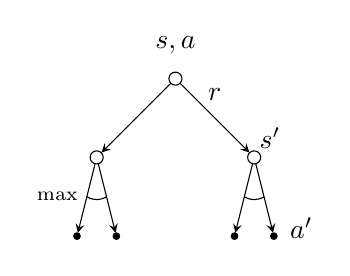
\begin{tikzpicture}
    \node[draw,circle,scale=1/2] (s) at (0,0) {};
    \node[above=1mm of s] {$s,a$};
    \node at (0.5, -0.2) {$r$};
    \foreach \x in {-1, 1} {
      \node[draw,circle,scale=1/2] (b\x) at (\x, -1) {};
      \node[draw,circle,fill,scale=1/4] (l\x) at (\x-.25,-2) {};
      \node[draw,circle,fill,scale=1/4] (r\x) at (\x+.25,-2) {};
      \draw[-stealth] (s) -- (b\x);
      \draw[-stealth] (b\x) -- (l\x);
      \draw[-stealth] (b\x) -- (r\x);
      \path[-] (\x+.125,-1.5) edge[bend left=30] (\x-.125,-1.5);
    }
    \node at (-1.5, -1.5) {\scriptsize max};
    \node at (1.2, -0.75) {$s'$};
    % \node[below = 2mm of b1] {$p$};
    \node at (1.6, -1.9) {$a'$};
    % \node at (-1.2, -0.5) {max};
    % \path[-] (-.25,-.25) edge[bend right=30] (.25, -.25);
  \end{tikzpicture}
\end{document}